\clearpage
\thispagestyle{empty}
\begin{landscape}
    \centering
    %\vspace*{\fill}
    \captionsetup{width=1.15\linewidth}
    \begin{figure}[!h]
        \centering
        \begin{tikzpicture}
        \begin{axis}[                                                                                                                     ticks=none,
            width=1.6\textheight,           
            height=\textwidth,    
            axis x line=center,                                                                            
            axis y line=center,
            xmin=-12.5,                                                                                                  
            xmax=12.5,
            ymin=-5,                                                                                                         
            ymax=5,
            xlabel={\LARGE $\Re{(p)}$},
            ylabel={\LARGE $\Im{(p)}$},
            xlabel style={right},
            ylabel style={above},                                                                                       
            ]      
            \draw [white!90!blue,fill=white!95!blue]   (axis cs:-12.5,-5) rectangle (axis cs:0,5);
            \draw [white!90!black,fill=white!90!black] (axis cs:0,-5) rectangle (axis cs:12.5,5);

            \draw [ultra thick,-latex]   (axis cs:-12.5,0) -- (axis cs:12.5,0);
            \draw [ultra thick,-latex]   (axis cs:0,-5) -- (axis cs:0,5);

            \coordinate (pt01) at (axis cs:-6.5,4.5);
            \coordinate (pt02) at (axis cs:6.5,4.5);

            \coordinate (pt1) at (axis cs:-12.5,2.0);
            \addplot[mark=x,black!60!green,ultra thick,only marks,mark size=7pt]  coordinates{ (-11,1.5) (-11,-1.5) } ;      
            \draw[ultra thick,dotted,color=black!60!green] (axis cs:-11,1.5) -- (axis cs:-11,-1.5) ;

            \coordinate (pt2) at (axis cs:-7,1.0);
            \addplot[mark=x,black!10!green,ultra thick,only marks,mark size=7pt]  coordinates{ (-5,0.5) (-5,-0.5) } ;  
            \draw[ultra thick,dotted,color=black!10!green] (axis cs:-5,0.5) -- (axis cs:-5,-0.5) ;

            \coordinate (pt3) at (axis cs:-10.25,-3.0);
            \addplot[mark=x,black!50!red,ultra thick,only marks,mark size=7pt]    coordinates{ (-8,0) } ;             

            \coordinate (pt4) at (axis cs:-4.75,-3.0);
            \addplot[mark=x,red,ultra thick,only marks,mark size=7pt]    coordinates{ (-2,0) } ;                      

            \coordinate (pt5) at  (axis cs:1.25,-5);
            \coordinate (pt52) at (axis cs:1.25,-3);
            \addplot[mark=x,black,ultra thick,only marks,mark size=7pt]  coordinates{ (0,0) } ;                      

            \coordinate (pt6) at (axis cs:1.25,2);
            \coordinate (pt62) at (axis cs:1.25,0);
            \addplot[mark=x,black!50!white,ultra thick,only marks,mark size=7pt]  coordinates{ (0,2) (0,-2) } ;              
            \draw[ultra thick,dotted,color=black!50!white] (axis cs:0,-2) to[bend right] (axis cs:0,2);

            \coordinate (pt7) at (axis cs:8.25,2);
            \addplot[mark=x,blue,ultra thick,only marks,mark size=7pt]   coordinates{ (11,1.5) (11,-1.5) } ;                
            \draw[ultra thick,dotted,color=blue] (axis cs:11,1.5) -- (axis cs:11,-1.5) ;

            \coordinate (pt8) at (axis cs:6.5,-3);
            \addplot[mark=x,orange,ultra thick,only marks,mark size=7pt] coordinates{ (8,0) } ;                  

        \end{axis}


            \node at (pt01) {\textbf{\Large STABLE}};
            \node at (pt02) {\textbf{\Large INSTABLE}};
            % pt1
            \node[anchor=south west] at (pt1) {
                \begin{tikzpicture}
                    \begin{axis}[
                    ticks=none,
                    width=4cm,    
                    height=4cm,    
                    axis x line=center,                                                                            
                    axis y line=center,
                    xmin=-0.5,                                                                                                                    xmax=6.5,
                    ymin=-0.5,                                                                        
                    ymax=2.5,
                    xlabel={$t$},
                    ylabel={$s(t)$},
                    xlabel style={below right},
                    ylabel style={right}
                    ]
                    \addplot [very thick,color=black!60!green,domain=0:10, samples=501,unbounded coords=jump]{1.2*sin(4.5*deg(x))*exp(-0.7*x)};
                    \addplot [thick,dotted,color=black,domain=0:10, samples=501,unbounded coords=jump]{1.2*exp(-0.7*x)+1};
                    \addplot [thick,dotted,color=black,domain=0:10, samples=501,unbounded coords=jump]{-1.2*exp(-0.7*x)+1};
                    \end{axis}
                \end{tikzpicture}
            };

            % pt2
            \node[anchor=south west] at (pt2) {
                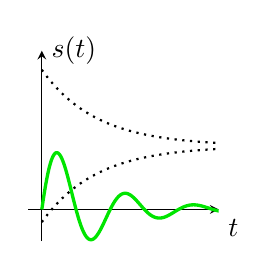
\begin{tikzpicture}
                    \begin{axis}[
                    ticks=none,
                    width=4cm,    
                    height=4cm,    
                    axis x line=center,                                                                            
                    axis y line=center,
                    xmin=-0.5,                                                                                                                    xmax=6.5,
                    ymin=-0.5,                                                                        
                    ymax=2.5,
                    xlabel={$t$},
                    ylabel={$s(t)$},
                    xlabel style={below right},
                    ylabel style={right}
                    ]
                    \addplot [very thick,color=black!10!green,domain=0:10, samples=501,unbounded coords=jump]{1.2*sin(2.5*deg(x))*exp(-0.5*x)};
                    \addplot [thick,dotted,color=black,domain=0:10, samples=501,unbounded coords=jump]{1.2*exp(-0.5*x)+1};
                    \addplot [thick,dotted,color=black,domain=0:10, samples=501,unbounded coords=jump]{-1.2*exp(-0.5*x)+1};
                    \end{axis}
                \end{tikzpicture}
            };
            % pt3
            \node[anchor=south west] at (pt3) {
                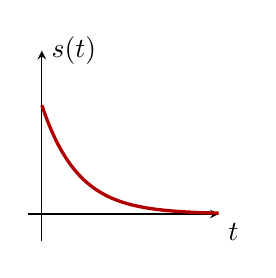
\begin{tikzpicture}
                    \begin{axis}[
                    ticks=none,
                    width=4cm,    
                    height=4cm,    
                    axis x line=center,                                                                            
                    axis y line=center,
                    xmin=-0.5,                                                                                                                    xmax=6.5,
                    ymin=-0.5,                                                                        
                    ymax=3,
                        xlabel={$t$},
                        ylabel={$s(t)$},
                    xlabel style={below right},
                    ylabel style={right}
                    ]
                    \addplot [very thick,color=black!30!red,domain=0:10, samples=501,unbounded coords=jump]{2*exp(-0.75*x)};
                    \end{axis}
                \end{tikzpicture}
            };
            % pt4
            \node[anchor=south west] at (pt4) {
                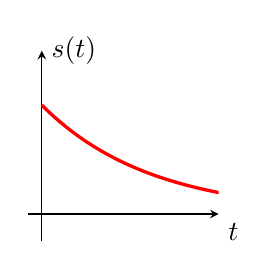
\begin{tikzpicture}
                    \begin{axis}[
                    ticks=none,
                    width=4cm,    
                    height=4cm,    
                    axis x line=center,                                                                            
                    axis y line=center,
                    xmin=-0.5,                                                                                                                    xmax=6.5,
                    ymin=-0.5,                                                                        
                    ymax=3,
                        xlabel={$t$},
                        ylabel={$s(t)$},
                    xlabel style={below right},
                    ylabel style={right}
                    ]
                    \addplot [very thick,color=red,domain=0:10, samples=501,unbounded coords=jump]{2*exp(-0.25*x)};
                    \end{axis}
                \end{tikzpicture}
            };
            % pt5
            \node[anchor=south west] at (pt5) {
                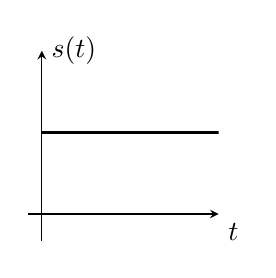
\begin{tikzpicture}
                    \begin{axis}[
                    ticks=none,
                    width=4cm,    
                    height=4cm,    
                    axis x line=center,                                                                            
                    axis y line=center,
                    xmin=-0.5,                                                                                                                    xmax=6.5,
                    ymin=-0.5,                                                                        
                    ymax=3,
                    xlabel={$t$},
                    ylabel={$s(t)$},
                    xlabel style={below right},
                    ylabel style={right}
                    ]
                    \addplot [very thick,color=black,domain=0:10, samples=501,unbounded coords=jump]{1.5};
                    \end{axis}
                \end{tikzpicture}
            };
            % pt52
            \node[anchor=south west] at (pt52) {
                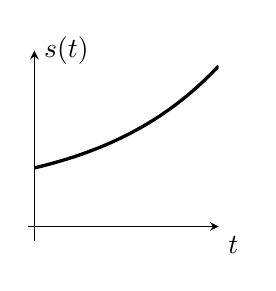
\begin{tikzpicture}
                    \begin{axis}[
                    ticks=none,
                    width=4cm,    
                    height=4cm,    
                    axis x line=center,                                                                            
                    axis y line=center,
                    xmin=-0.5,                                                                                                                    xmax=15,
                    ymin=-0.5,                                                                        
                    ymax=6,
                    xlabel={$t$},
                    ylabel={$s(t)$},
                    xlabel style={below right},
                    ylabel style={right}
                    ]
                    \addplot [very thick,color=black,domain=0:15, samples=501,unbounded coords=jump]{1+exp(0.1*x)};
                    \end{axis}
            \end{tikzpicture}
            };
            % pt6
            \node[anchor=south west] at (pt6) {
                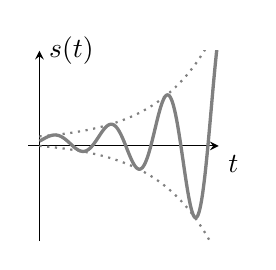
\begin{tikzpicture}
                    \begin{axis}[
                    ticks=none,
                    width=4cm,    
                    height=4cm,    
                    axis x line=center,                                                                            
                    axis y line=center,
                    xmin=-0.5,                                                                                                                    xmax=8,
                    ymin=-20,                                                                        
                    ymax=20,
                    xlabel={$t$},
                    ylabel={$s(t)$},
                    xlabel style={below right},
                    ylabel style={right}
                    ]
              \addplot [very thick,color=black!50!white,domain=0:10, samples=501,unbounded coords=jump]{sin(2.5*deg(x))*exp(0.40*x)+1};
              \addplot [thick,dotted,color=black!50!white,domain=0:10, samples=501,unbounded coords=jump]{ exp(0.4*x)+1};
              \addplot [thick,dotted,color=black!50!white,domain=0:10, samples=501,unbounded coords=jump]{-exp(0.4*x)+1};
                    \end{axis}
                \end{tikzpicture}
            };
            % pt62
            \node[anchor=south west] at (pt62) {
                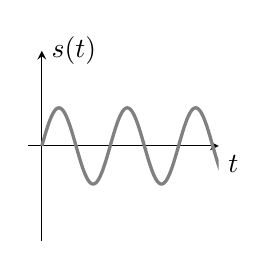
\begin{tikzpicture}
                    \begin{axis}[
                    ticks=none,
                    width=4cm,    
                    height=4cm,    
                    axis x line=center,                                                                            
                    axis y line=center,
                    xmin=-0.5,                                                                                                                    xmax=6.5,
                    ymin=-2.5,                                                                        
                    ymax=2.5,
                    xlabel={$t$},
                    ylabel={$s(t)$},
                    xlabel style={below right},
                    ylabel style={right}
                    ]
                    \addplot [very thick,color=black!50!white,domain=0:10, samples=501,unbounded coords=jump]{sin(2.5*deg(x))};
                    \end{axis}
                \end{tikzpicture}
            };
            % pt7
            \node[anchor=south west] at (pt7) {
                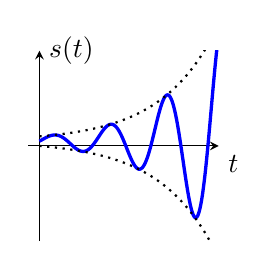
\begin{tikzpicture}
                    \begin{axis}[
                    ticks=none,
                    width=4cm,    
                    height=4cm,    
                    axis x line=center,                                                                            
                    axis y line=center,
                    xmin=-0.5,                                                                                                                    xmax=8.0,
                    ymin=-20,                                                                        
                    ymax=20,
                    xlabel={$t$},
                    ylabel={$s(t)$},
                    xlabel style={below right},
                    ylabel style={right}
                    ]
              \addplot [very thick,color=blue,domain=0:10, samples=501,unbounded coords=jump]{sin(2.5*deg(x))*exp(0.40*x)+1};
              \addplot [thick,dotted,color=black,domain=0:10, samples=501,unbounded coords=jump]{ exp(0.4*x)+1};
              \addplot [thick,dotted,color=black,domain=0:10, samples=501,unbounded coords=jump]{-exp(0.4*x)+1};
                    \end{axis}
              \end{tikzpicture}
            };
            % pt8
            \node[anchor=south west] at (pt8) {
                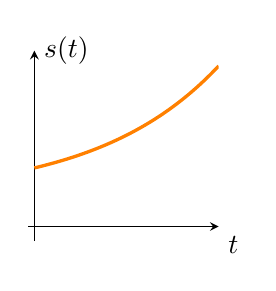
\begin{tikzpicture}
                    \begin{axis}[
                    ticks=none,
                    width=4cm,    
                    height=4cm,    
                    axis x line=center,                                                                            
                    axis y line=center,
                    xmin=-0.5,                                                                                                                    xmax=15,
                    ymin=-0.5,                                                                        
                    ymax=6,
                    xlabel={$t$},
                    ylabel={$s(t)$},
                    xlabel style={below right},
                    ylabel style={right}
                    ]
                    \addplot[very thick,color=orange,domain=0:15,samples=501,unbounded coords=jump]{1+exp(0.1*x)};
                    \end{axis}
                \end{tikzpicture}
            };
        \end{tikzpicture}
    \caption{Stabilité d'un SLCI d'après la carte des pôles de sa fonction de transfert et de leurs
    réponses impulsionnelles.
    (Vert) Deux pôles complexes conjugués. 
    (Rouge) Pôle à partie réel négative. 
    (Gris) Deux pôles complexes conjugués à partie réelle nulle.
    (Noir) Pôle nul.
    (Bleu) Deux pôles complexes conjugués à partie réelle positive.
    (Orange) Pôle à partie réel positive.}
    \end{figure}
%    %\vfill
\end{landscape}

\clearpage
\pagestyle{fancy}
\captionsetup{width=0.8\linewidth}
